\documentclass{aa}
\usepackage[varg]{txfonts}
\usepackage{siunitx}
\usepackage[version=3]{mhchem}

\begin{document}


\title{NIR spectroscopy of the Sun and HD20010}
\subtitle{Compiling a new linelist in the NIR}

\subtitle{}

\author{Andreasen, D. T.\inst{\ref{inst1}, \ref{inst2}} \and
        Santos, N.\inst{\ref{inst1}} \and
        Sousa, S.\inst{\ref{inst1}} \and
        Delgado-Mena, E.\inst{\ref{inst1}}}

\institute{%
    Centro de Astrofísica da Universidade do Porto,
    Rua das Estrelas, 4150-762 Porto, Portugal
    \email{daniel.andreasen@astro.up.pt}\label{inst1}
        \and
    Departamento de F\'iseca e Astronomia, Faculdade de Ci\^encias, Universidade do Porto,
    Rua do Campro Alegre, 4169-007 Porto, Portugal\label{inst2}
}


\date{\today}

\abstract{}{}{}{}



\keywords{data reduction: high resolution spectra -- data reduction: low
    resolution spectra -- stars individual: HD20010 -- stars individual: Sun}
\maketitle



\section{Introduction}
\label{sec:introduction}
Effective surface temperature ($T_\mathrm{eff}$), surface gravity ($\log g$),
and metallicity ([Fe/H], where iron is used as a proxy) are fundamental
atmospheric parameters necessary to characterise a star, as well to determine
other inderict fundamental parameters, such as mass, radius, and age from
stellar evolutionary models \citep{Girardi2000}.

Precise and accurate stellar parameters are also essential in exoplanet
searches. Planetary radius, and mass are mainly found from lightcurve analysis and
radial velocity analysis, respectively. These parameters are related to the
stellar parameters.




% In this seminar I will explore the use of NIR spectroscopy towards the
% derivation of precise parameters for FGK dwarfs. This work will serve as a
% first approach to the determination of parameters in this spectral domain,
% using well known FGK dwarfs as benchmarks. NIR stellar spectra are
% significantly less blended, thus allowing for a precise line-by-line analysis
% \citep{Woolf2006,2012Onehag}. The NIR domain will then be key to solve the
% problem of M-dwarf parameter estimation. Note that the IR part of the spectrum
% is preferred over the optical for M-dwarfs because there is less photospheric
% molecular line blending and continuum depression.
%
% For the determination of stellar parameters we need to choose our approach. In
% general there is two widely used approaches to analyse spectra, 1: The
% spectral synthesis method, and 2: The equivalent method. I will use the latter
% approach.

\section{The method}
\label{sec:the_method}
Generally speaking there are two methods for determining parameters from a
spectrum.  One is the spectral synthesis method, where a synthetic spectrum is
created and by minimization procedure a best fit is found bewteen the synthetic
spectrum and the real spectrum. The stellar parameters are give from the input
to the synthetic spectrum.

The other method is the equivalent width (EW) method, which we use in this
work.  With this method the EW are measured for all lines in a line list. The
EW is given as
\begin{align}
    \label{eq:EW}
    EW = \int_0^\infty \left(1 - \frac{F_\lambda}{F_0}\right) d\lambda,
\end{align}
where $F_0$ is the continuum level and $F_\lambda$ is is the flux as a function
of wavelength. In other words, the EW width is the area from a spectral line up
to the normalized continuum level.

With the EW the abundance for individual lines can be found with a code like
MOOG\footnote{The MOOG code can be downloaded free at
\url{http://www.as.utexas.edu/~chris/moog.html}}. By changing atmospheric
parameters as input for MOOG, similar abundances will be achieved for similar
elements when the right atmospheric parameters are chosen. Here we use neutral
iron and single ionized iron: FeI and FeII, respectively.

A disadvantage for this method, and a general problem with spectroscopy, is the
determination of the continuum flux level. Misplacement of the continuum leads
to wrong measurements of the EW. Many spectroscopic features make it difficult
to determine the continuum. This is especially true for cool stars in the
optical where molecular depression and line blending is an issue. By moving the
analysis to the NIR, we reduce the molecular depression, and cooler stars line
M-dwarfs emit more in this spectral region, why the continuum is at least
easier to determine.

We look at the spectral region covered by the J, H, and K bands, which cover a
spectral region larger than $\SI{15000}{\AA}$.



% The final stellar parameters are obtained when no correlation is present
% \citep{Gray2006}. The iron abundance is derived in this process, computed by
% the mean abundance given by all lines analysed.




\subsection{Compiling the line list}
All iron lines with atomic line data were downloaded from the
VALD database\footnote{The VALD database can be found here:
\url{http://vald.astro.univie.ac.at/~vald3/php/vald.php}}. In total
78537 lines of FeI and FeII are present in the spectral region (FeI:
50198 and FeII: 28339). Many of these lines are to faint to see in a
spectrum. To select the lines for the line list a spectrum of the Sun
is used downloaded from the BASS2000 web page\footnote{The web page can
be found here: \url{bass2000.obspm.fr/solar_spect.php}}. The spectrum
were downloaded in the highest possible resolution. Since the resolution
is not constant the entire spectrum were interpolated to a regular grid
with constant wavelength step of $\SI{0.01}{\AA}$.

With the spectrum on a regular wavelength grid the
EW for all the lines were measured using the ARES
software\footnote{The ARES software can be found here:
\url{http://www.astro.up.pt/~sousasag/ares/}}\citep{Sousa2007}. This
software can measure EW automatically by fitting a Gaussian profile to
a spectral line. For a given line ARES output the central wavelength of
the line, the number of lines fitted for the end result, the depth of
the line, the FWHM of the line, the EW of the line, and last Gaussians
coefficients for the line.

We remove lines from the line list based criteria listed below:
\begin{itemize}
    \item If the number of fitted lines for a given line is higher than 10,
        this line is rejected because it is believed to be severely blended.
    \item If the EW is lower than $\SI{5}{m\AA}$ for a given line, the strength
        is too low and may be difficult to see in spectra with low S/N or a
        spectrum with many spectral features.
    \item If the EW is higher than $\SI{200}{m\AA}$ for a give line, the strength
        is too high and non-LTE effects is present in the core of the line.
    \item If the fitted central wavelength is more than $\SI{0.05}{\AA}$ away
        from the wavelength provided by VALD, the line will also be rejected to
        avoid false identification.
\end{itemize}




\subsection{Manually removal of lines}
\label{sub:manually_removal_of_lines}
At this step we reduced the number of lines to 6060 and 2735 for FeI and FeII
respectively. A manual inspection of the lines is necessary at this point in
order to sort bad lines.  We only removed lines where we were certain they did
not belong to either FeI or FeII from our list. The rest were kept as they
would appear as outliers later on in the analysis.

For the remaining iron lines, all lines from all elements in a small window
where downloaded. Again iron lines were removed from the list, if another
element fitted the absorption line better. Some iron lines were marked for
further investigation while the rest were kept in the line list.



\subsubsection{Synthesis of selected lines}
\label{sub:synthesis_of_selected_lines}
Lines from all elements in a small window around an iron line marked
for further investigation were used to make a synthetic spectra.
The synthetic spectra were made with MOOG. We used 3 different iron
abundances for the synthesis. One with solar iron abundance, and
then two $\pm0.2$ dex. If the synthetic spectra shows variation at
the absorption line of interest with respect to the different iron
abundances, then it's likely to be an iron line. We also changed
abundances of other elements in the proximity to see if our line is
blended with other elements.

Sometimes more than 1 iron line might be present with very similar
wavelengths. In order to find the iron line which is creating the
absorption line, one of the two were removed from the line list for
the synthetic spectra. If this removed (either fully or partially) the
absorption line in the synthetic spectra, then it will be the cause for
the real absorption line.

A few times two iron lines had similar wavelengths and excitation
potential. In those cases the $\log \mathrm{gf}$ were combined. First
converted to $\mathrm{gf}$, then an average value, and finally back to
$\log \mathrm{gf}$.


\subsubsection{Recalibrating the atomic data}
\label{ssub:Recalibrating-the-atomic-data}
The abundances were calculated for all lines with a atmosphere model
characterised by $T_\mathrm{eff}=\SI{5777}{K}$, $\log g = 4.438$,
$[Fe/H] = 0.0$, and $\xi_\mathrm{micro} = \SI{1.0}{km/s}$ to resemble
the Sun. Lines which have abundances that deviates more than 1 dex were
discarded For the Sun an iron abundance at 7.47 is considered according
to \citet{Gonzales2000}. At this point we are down to 319 and 12 lines,
respectively for Fe I and Fe II. We only removed Fe I lines here, since
the Fe II lines are sparse and important to determine the surface
gravity.

After the removal of lines from the complete VALD line list we
only need to recalibrate the lines. This is a common thing to do
for a star we know well \citep{2012Onehag}. Here we calculate the
abundance for line to line. If the abundance does not match the
Solar abundance, the $\log \mathrm{gf}$ were changed until it does.
The abundance varies more or less linearly with $\log \mathrm{gf}$.
Therefore the recalibrated $\log \mathrm{gf}$ can be found with few
iterations. In Figure~\ref{fig:Fe1_before_recal} the EW of the Fe I
lines are plotted with respect to the excitation potential. On top
of that, the color scale represent the abundance calculated before
the recalibration of $\log \mathrm{gf}$. A similar plot is seen in
Figure\ref{fig:Fe1_after_recal} but after the recalibration. Here the
abundance of all the lines are 7.47, why there is no color scale over
plotted.

\begin{figure}[htpb]
    \centering
    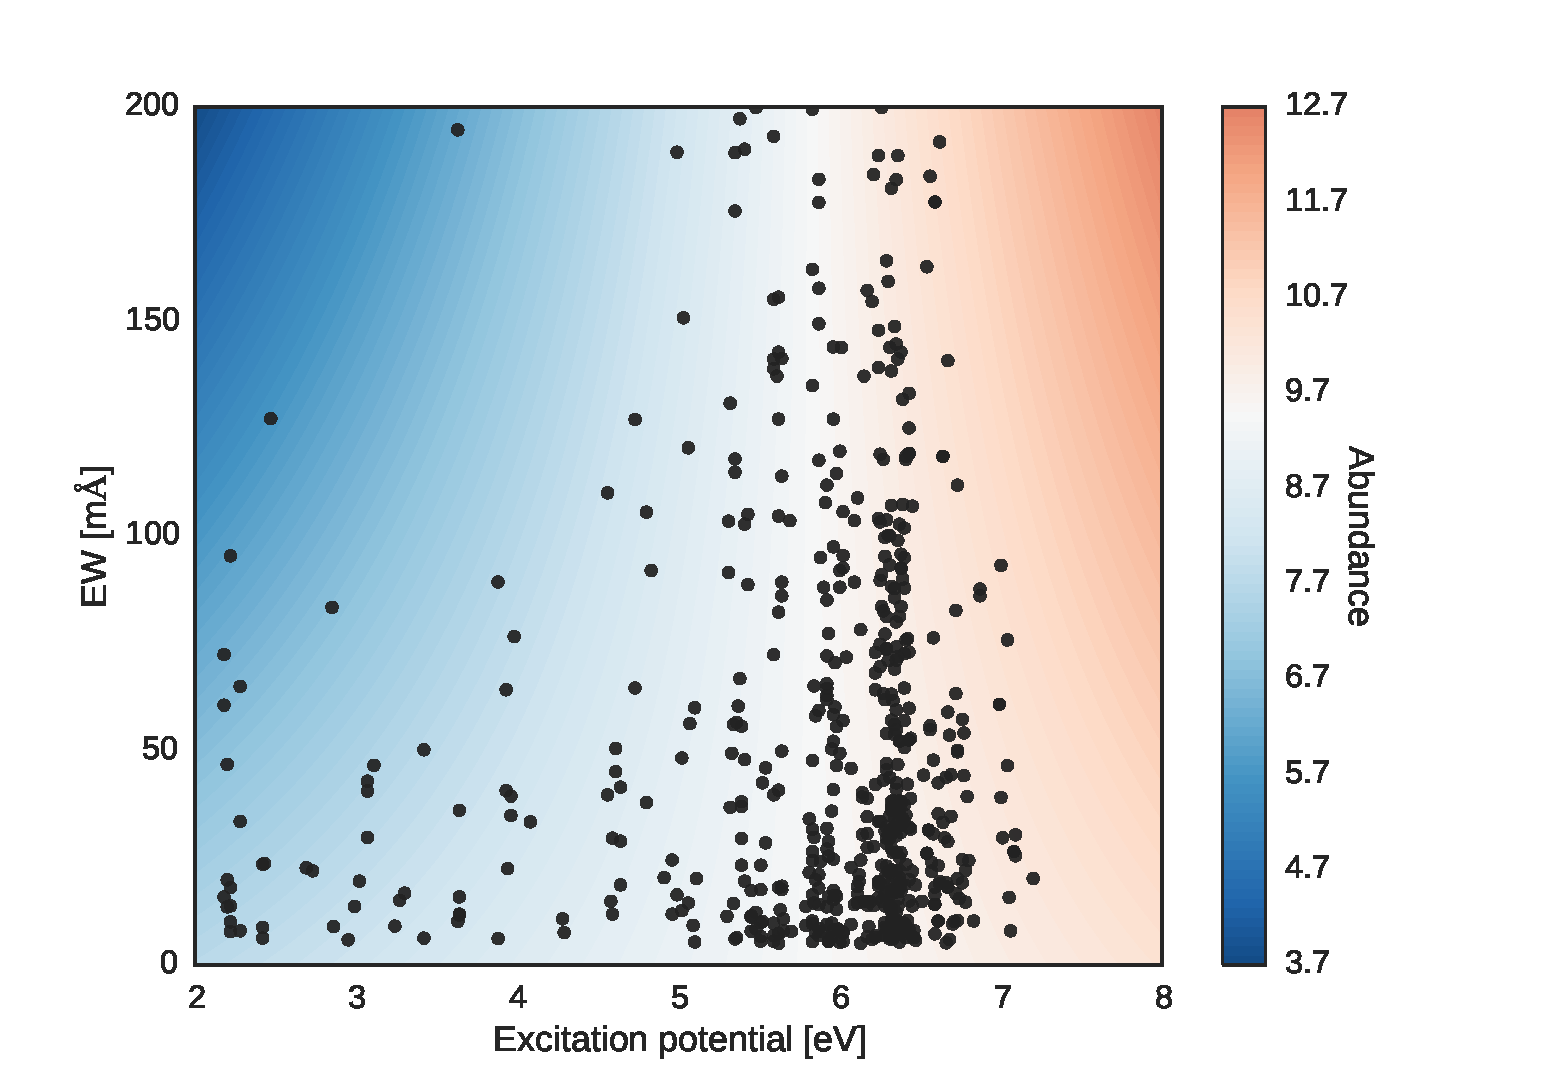
\includegraphics[width=0.9\linewidth]{figures/EWvsEP.pdf}
    \caption{The distribution of Fe I lines with. At the x axis is the
    excitation potential, while the measure EW is shown at the y axis. The
    color scale indicates the abundance before recalibration.}
    \label{fig:Fe1_before_recal}
\end{figure}


\begin{figure}[htpb]
    \centering
    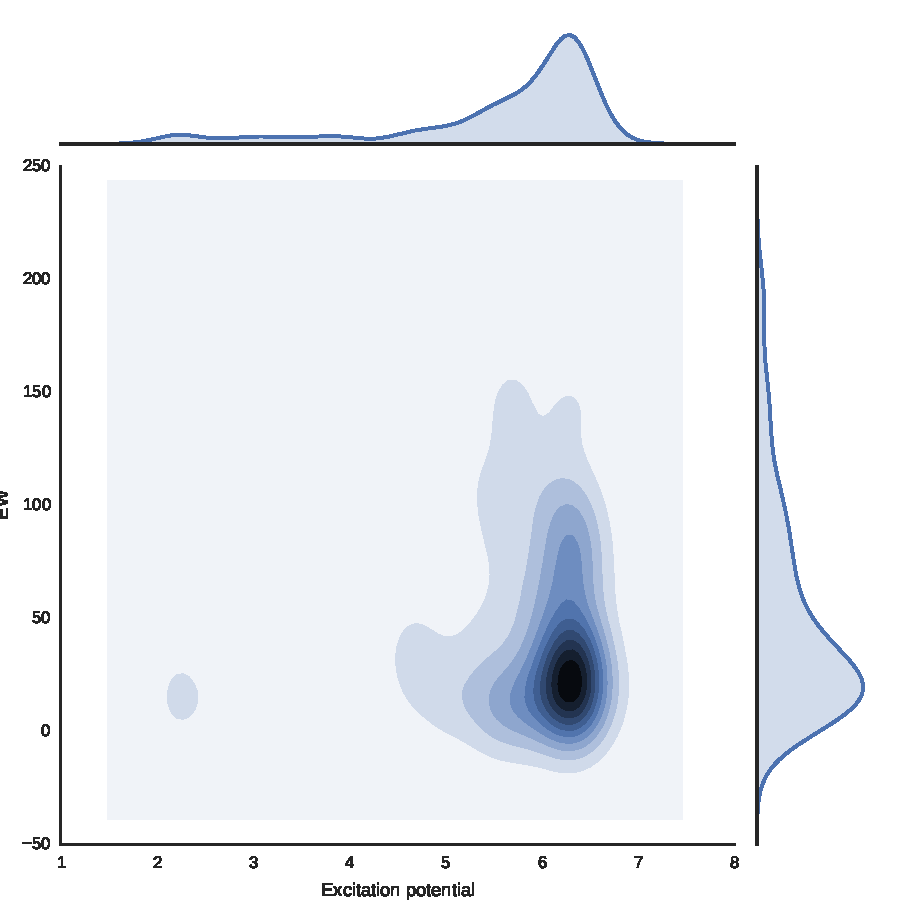
\includegraphics[width=0.9\linewidth]{figures/EWvsEP_cut.pdf}
    \caption{The distribution of Fe I lines with. At the x axis is the
    excitation potential, while the measure EW is shown at the y axis.
    The histograms at the top and to the right of the plot, show the
    distribution of the respective axis.}
    \label{fig:Fe1_after_recal}
\end{figure}



\section{Derived parameters of the Sun}
\label{sec:derived_parameters_of_the_sun}
We derive atmospheric parameters for the Sun with the recalibrated line list.
This is a trivial case since the line list is calibrated for the Sun, but it
serve as a consistency test. Additionally we added noise to the EW measurements
and derived parameters with different cuts in excitation potential (EP). We cut
in EP since the absorption lines are generally weaker, thus the relative error
in EW becomes higher. We want to avoid this in other stars. In
Figure~\ref{fig:solar_parameters} the parameters is plotted with different EP
cuts in the line list. The horizontal black line is the derived atmospheric
parameters without noise added to the EW.

\begin{figure}[htpb]
    \centering
    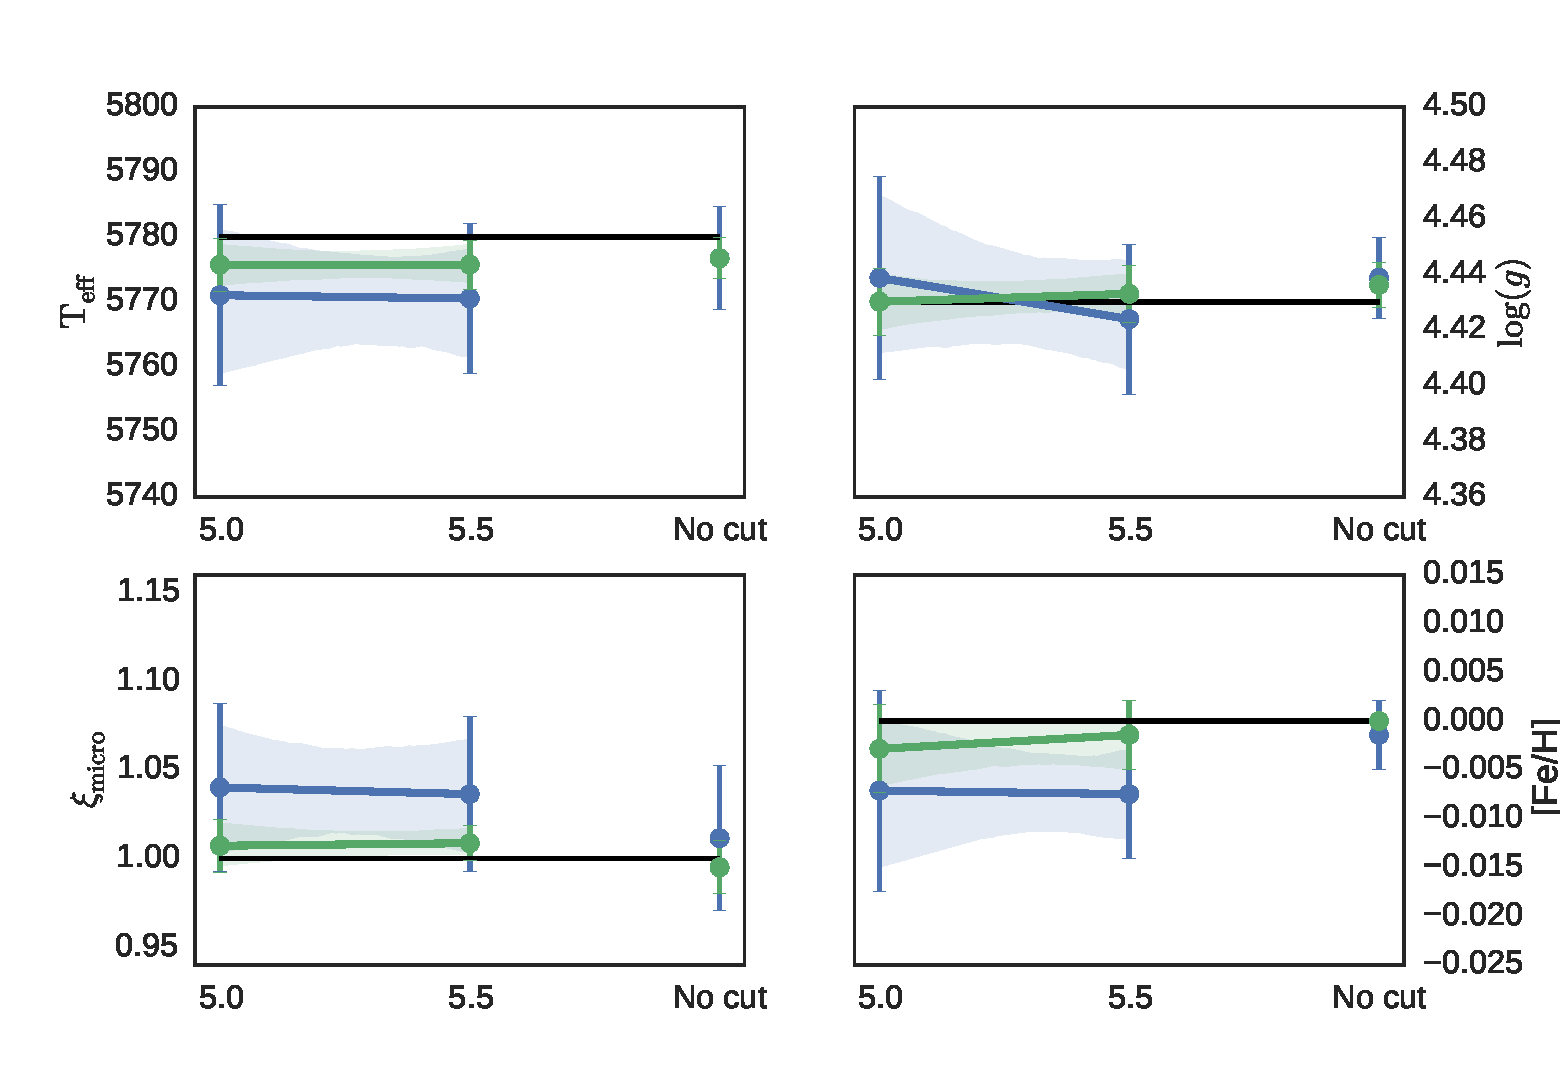
\includegraphics[width=0.9\linewidth]{figures/solar_parameters_10runs.pdf}
    \caption{Derived atmospheric parameters for the Sun. The horizontal black
    line is the parameters for the calibrated line list. The three points shows
    the median value of 10 runs with random noise added. The blue point is the
    result for the whole line list, while the two green points is the result
    from line lists cutted in EP as given on the x-axis.}
    \label{fig:solar_parameters}
\end{figure}

We calculate the atmospheric parameters, $\{T_\mathrm{eff}, \log
g, \xi_\mathrm{micro}, [\mathrm{Fe/H}]\}$, by adding noise to the
calibrated line list. This is done 10 times, and for each time, we use
the full line list, a line list with a cut in EP at $\SI{5.5}{eV}$, and
a line list with a cut in EP at $\SI{5.0}{eV}$. This gives a total of
31 line list for which we calculate the atmospheric parameters given
above. This are all plotted in Figure~\ref{fig:solar_parameters}. The
horizontal black line corresponds to the calibrated line list with no
noise added, i.e. the true solar parameters.

By adding noise to the EW measurements and calculate the atmospheric
parameters with different cuts in EP, we see how we over estimate all
the parameters except the iron abundance, when a cut in EP is not
applied. This suggest that it might be necessary to do a cut in the line
list for other stars to get reliable parameters. This is indeed the case
for HD20010.



\section{Derived parameters of HD20010}
\label{sec:derived_parameters_of_hd20010}

HD20010 is a well studied F8 subgiant, see e.g.
\cite{Mortier2013,lebzelter2012}. Therefore it is a prime object for our
studies, since we want to benchmark results from our new line list with
literature values.



\begin{figure}[htpb]
    \centering
    \includegraphics[width=0.9\linewidth]{figures/HD20010_parameters_cuts.pdf}
    \caption{atmospheric parameters for HD20010. In the top panel is the
    effective temperature. The middle panel is the iron abundance, and the
    bottom panel is the micro turbulence. The parameters are derived with
    different cuts in EP. The parameters for the full line list is plotted
    to the right for all three plots.}
    \label{fig:HD20010_parameters_cuts}
\end{figure}











\newpage
\bibliography{thesis}
\bibliographystyle{astron}
\nocite*{}

\end{document}



















\section{Summary}
\label{sec:conclusion}
It is a lengthy process to compile a final good line list for spectral
analysis, and with a high possibility to make errors along the way. E.g.\ the
data that was first used from the \url{vso.nso.edu} was not corrected in radial
velocity was used. This was only discovered by an accident after many of the
above steps were already taken. Therefore all the steps needed to be done
again, after switching to the BASS2000 dataset.

Now the solar spectrum are ready for analysis. All the neutral and first
ionized iron lines in a wide wavelength coverage in the NIR have been
downloaded from the VALD database. With the lines follows the excitation
potential and the oscillator strength. The latter has to be recalibrated for
all the lines before an analysis can take place.

Far from all the lines from the VALD database are useful for a spectral
analysis in the NIR domain. Therefore many of the lines have been removed
following the selection criteria in Section~\ref{ssec:compiling_the_line_list}.

\subsubsection{The future work}
\label{ssub:the_future_work}
At the moment of writing the next step is to remove ``false-positive'' lines,
which are lines there are found in the VALD database and seems to hit a
spectral line, but in reality the spectral line belongs to another element.
This step has to be done before recalibrating the $\log gf$ values makes sense.
Even though yet another somewhat lengthy process awaits ahead, the
recalibration software is ready, as it was already shown in
Figure~\ref{fig:recalFe1}.

The recalibration will be done with respect to the Sun, the star we know best.
The goal is to characterise M-dwarfs, but since the Sun (G2V by definition,
\citet{Gray2006}) is not far away in spectral class, it should be save to use
the Sun as a starting point. However, for benchmarking the line list a sample
of FGK-dwarfs will be analysed. These stars will have well known stellar
parameters in order to test the line list. After the benchmarking some small
corrections might be made to the line list, in order to have consistent
results.

This will be the final step before the determination of stellar parameters
using iron lines in the NIR combined with the equivalent method on M-dwarfs,
and the characterisation of this cool planet hosts.


